  \section[SPARQL Protocol and RDF Query Language (SPARQL)]{SPARQL}
  \label{sec:sparql}

  \initial{S}\textit{SPARQL Protocol and RDF Query Language (SPARQL)}\
  is a W3C recommend standard for querying RDF data.\
  It allows one to query remote RDF resources, in a manner similar to the querying of databases using SQL.\
  A SPARQL query is a set of graph patterns; any data triple matching these patterns is added to the query results. \citep{Jarrar_mashql:_2008}\\     

  \subsection{Why use it}

By having the ability to query the RDF data, you will be able to enhance quality of clinical research and patient care by finding new insights in healthcare. Data is no good just on it's own, you need a tool available to easily analyze it and SPARQL is this tool.
		
  \subsection{Alternatives}

  SquishQL - A simple RDF query language for beginners that allows for SQL syntax. Has very little adoption compared to the more powerful query language SPARQL  \citep{_Mikhalenko_2013}\

  \subsection{Examples}
  \begin{figure}[h!]
    \begin{subfigure}[b]{.5\linewidth}
      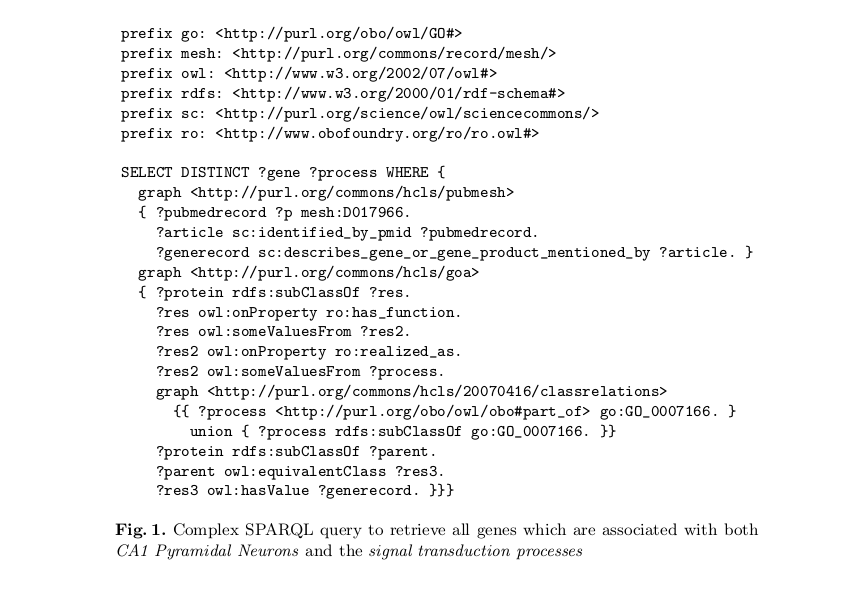
\includegraphics[width=1.2\textwidth]{sparql1.png}
      \caption{SPARQL Query 1}
      \label{fig:first}
    \end{subfigure}
    ~
    \begin{subfigure}[b]{.5\linewidth}
      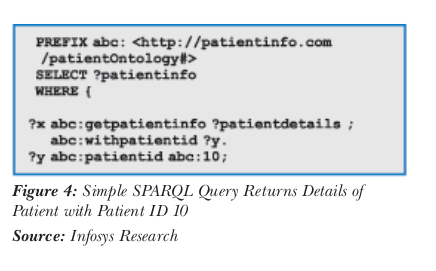
\includegraphics[width=1.2\textwidth]{sparqlh.png}
      \caption{SPARQL Query 2}
      \label{fig:second}
    \end{subfigure}
    \caption{Examples}
    \label{fig:sparql_examples}
  \end{figure}

  \noindent The first and second subfigures in subfigure\
  1 are labeled as\
  \ref{fig:first} \cite{stenzhorn2008simplifying}\
  and \ref{fig:second}  \cite{parachuri2008role} respectively.\\
